\documentclass[11pt,preprint, authoryear]{elsarticle}

\usepackage{lmodern}
%%%% My spacing
\usepackage{setspace}
\setstretch{1.5}
\DeclareMathSizes{12}{14}{10}{10}

% Wrap around which gives all figures included the [H] command, or places it "here". This can be tedious to code in Rmarkdown.
\usepackage{float}
\let\origfigure\figure
\let\endorigfigure\endfigure
\renewenvironment{figure}[1][2] {
    \expandafter\origfigure\expandafter[H]
} {
    \endorigfigure
}

\let\origtable\table
\let\endorigtable\endtable
\renewenvironment{table}[1][2] {
    \expandafter\origtable\expandafter[H]
} {
    \endorigtable
}


\usepackage{ifxetex,ifluatex}
\usepackage{fixltx2e} % provides \textsubscript
\ifnum 0\ifxetex 1\fi\ifluatex 1\fi=0 % if pdftex
  \usepackage[T1]{fontenc}
  \usepackage[utf8]{inputenc}
\else % if luatex or xelatex
  \ifxetex
    \usepackage{mathspec}
    \usepackage{xltxtra,xunicode}
  \else
    \usepackage{fontspec}
  \fi
  \defaultfontfeatures{Mapping=tex-text,Scale=MatchLowercase}
  \newcommand{\euro}{€}
\fi

\usepackage{amssymb, amsmath, amsthm, amsfonts}

\def\bibsection{\section*{References}} %%% Make "References" appear before bibliography


\usepackage[round]{natbib}

\usepackage{longtable}
\usepackage[margin=2.3cm,bottom=2cm,top=2.5cm, includefoot]{geometry}
\usepackage{fancyhdr}
\usepackage[bottom, hang, flushmargin]{footmisc}
\usepackage{graphicx}
\numberwithin{equation}{section}
\numberwithin{figure}{section}
\numberwithin{table}{section}
\setlength{\parindent}{0cm}
\setlength{\parskip}{1.3ex plus 0.5ex minus 0.3ex}
\usepackage{textcomp}
\renewcommand{\headrulewidth}{0.2pt}
\renewcommand{\footrulewidth}{0.3pt}

\usepackage{array}
\newcolumntype{x}[1]{>{\centering\arraybackslash\hspace{0pt}}p{#1}}

%%%%  Remove the "preprint submitted to" part. Don't worry about this either, it just looks better without it:
\makeatletter
\def\ps@pprintTitle{%
  \let\@oddhead\@empty
  \let\@evenhead\@empty
  \let\@oddfoot\@empty
  \let\@evenfoot\@oddfoot
}
\makeatother

 \def\tightlist{} % This allows for subbullets!

\usepackage{hyperref}
\hypersetup{breaklinks=true,
            bookmarks=true,
            colorlinks=true,
            citecolor=blue,
            urlcolor=blue,
            linkcolor=blue,
            pdfborder={0 0 0}}


% The following packages allow huxtable to work:
\usepackage{siunitx}
\usepackage{multirow}
\usepackage{hhline}
\usepackage{calc}
\usepackage{tabularx}
\usepackage{booktabs}
\usepackage{caption}


\newenvironment{columns}[1][]{}{}

\newenvironment{column}[1]{\begin{minipage}{#1}\ignorespaces}{%
\end{minipage}
\ifhmode\unskip\fi
\aftergroup\useignorespacesandallpars}

\def\useignorespacesandallpars#1\ignorespaces\fi{%
#1\fi\ignorespacesandallpars}

\makeatletter
\def\ignorespacesandallpars{%
  \@ifnextchar\par
    {\expandafter\ignorespacesandallpars\@gobble}%
    {}%
}
\makeatother

\newenvironment{CSLReferences}[2]{%
}

\urlstyle{same}  % don't use monospace font for urls
\setlength{\parindent}{0pt}
\setlength{\parskip}{6pt plus 2pt minus 1pt}
\setlength{\emergencystretch}{3em}  % prevent overfull lines
\setcounter{secnumdepth}{5}

%%% Use protect on footnotes to avoid problems with footnotes in titles
\let\rmarkdownfootnote\footnote%
\def\footnote{\protect\rmarkdownfootnote}
\IfFileExists{upquote.sty}{\usepackage{upquote}}{}

%%% Include extra packages specified by user

%%% Hard setting column skips for reports - this ensures greater consistency and control over the length settings in the document.
%% page layout
%% paragraphs
\setlength{\baselineskip}{12pt plus 0pt minus 0pt}
\setlength{\parskip}{12pt plus 0pt minus 0pt}
\setlength{\parindent}{0pt plus 0pt minus 0pt}
%% floats
\setlength{\floatsep}{12pt plus 0 pt minus 0pt}
\setlength{\textfloatsep}{20pt plus 0pt minus 0pt}
\setlength{\intextsep}{14pt plus 0pt minus 0pt}
\setlength{\dbltextfloatsep}{20pt plus 0pt minus 0pt}
\setlength{\dblfloatsep}{14pt plus 0pt minus 0pt}
%% maths
\setlength{\abovedisplayskip}{12pt plus 0pt minus 0pt}
\setlength{\belowdisplayskip}{12pt plus 0pt minus 0pt}
%% lists
\setlength{\topsep}{10pt plus 0pt minus 0pt}
\setlength{\partopsep}{3pt plus 0pt minus 0pt}
\setlength{\itemsep}{5pt plus 0pt minus 0pt}
\setlength{\labelsep}{8mm plus 0mm minus 0mm}
\setlength{\parsep}{\the\parskip}
\setlength{\listparindent}{\the\parindent}
%% verbatim
\setlength{\fboxsep}{5pt plus 0pt minus 0pt}



\begin{document}



\begin{frontmatter}  %

\title{Olympics: Insights for a TV Station in New Delhi}

% Set to FALSE if wanting to remove title (for submission)




\author[Add1]{Angela Euston-Brown\footnote{\textbf{Contributions:}
  \newline \emph{The student would like to thank the Olympics organiser
  for the data and Nico Katzke for the skills.}}}
\ead{28784618@sun.ac.za}





\address[Add1]{Stellenbosch University, Stellenbosch, South Africa}

\cortext[cor]{Corresponding author: Angela Euston-Brown\footnote{\textbf{Contributions:}
  \newline \emph{The student would like to thank the Olympics organiser
  for the data and Nico Katzke for the skills.}}}

\begin{abstract}
\small{
The Summer Olympics are soon to be held in Paris this year. This
document explores how India has historically done in the Olympics, as
well as which countries have dominated and which have surprised us all.
These findings form the solution for Question 4 of the datascience exam.
}
\end{abstract}

\vspace{1cm}





\vspace{0.5cm}

\end{frontmatter}

\setcounter{footnote}{0}



%________________________
% Header and Footers
%%%%%%%%%%%%%%%%%%%%%%%%%%%%%%%%%
\pagestyle{fancy}
\chead{}
\rhead{}
\lfoot{}
\rfoot{\footnotesize Page \thepage}
\lhead{}
%\rfoot{\footnotesize Page \thepage } % "e.g. Page 2"
\cfoot{}

%\setlength\headheight{30pt}
%%%%%%%%%%%%%%%%%%%%%%%%%%%%%%%%%
%________________________

\headsep 35pt % So that header does not go over title




\hypertarget{indias-comparative-performance}{%
\section{\texorpdfstring{India's Comparative Performance
\label{India}}{India's Comparative Performance }}\label{indias-comparative-performance}}

Figure \ref{Figure1} produced below compares the total number of medals
won in the Summer Olympics by India and similar sized economies,
emerging market economies and South American countries. Each dot also
captures the country's GDP per capita in its size.

The plot shows that:

\begin{itemize}
\item
  India compares relatively favourably to countries with a similar
  economy, based on GDP per capita. However, Kenya outstrips India's
  medal winnings despite a lower GDP per Capita. Ukraine's total medal
  winnings similarly outsrip India's, but their GDP is marginally
  larger. India has the 3rd highest number of medals amongst those with
  similar GDP per Capita.
\item
  India's total medals one is much lower than other emerging market
  economies (emerging market economies identified using sources
  (\protect\hyperlink{ref-sankaran2021does}{Sankaran, Krishna \&
  Vadivel, 2021})). However, this does appear to be somewhat captured by
  the relative GDP per Capita within the group, with India having the
  lowest GDP per Capita. India's performance is comparable to that of
  Indonesia, despite a lower GDP per Capita.
\item
  In comparison to selected South American countries (that are not
  considered an emerging market economy such as Brazil and Argentina),
  India performs well despite having lower GDP per Capita. In fact,
  despite having the lowest GDP per capita amongst this grouping, India
  has the highest total number of medals won.
\end{itemize}

\begin{figure}[H]

{\centering 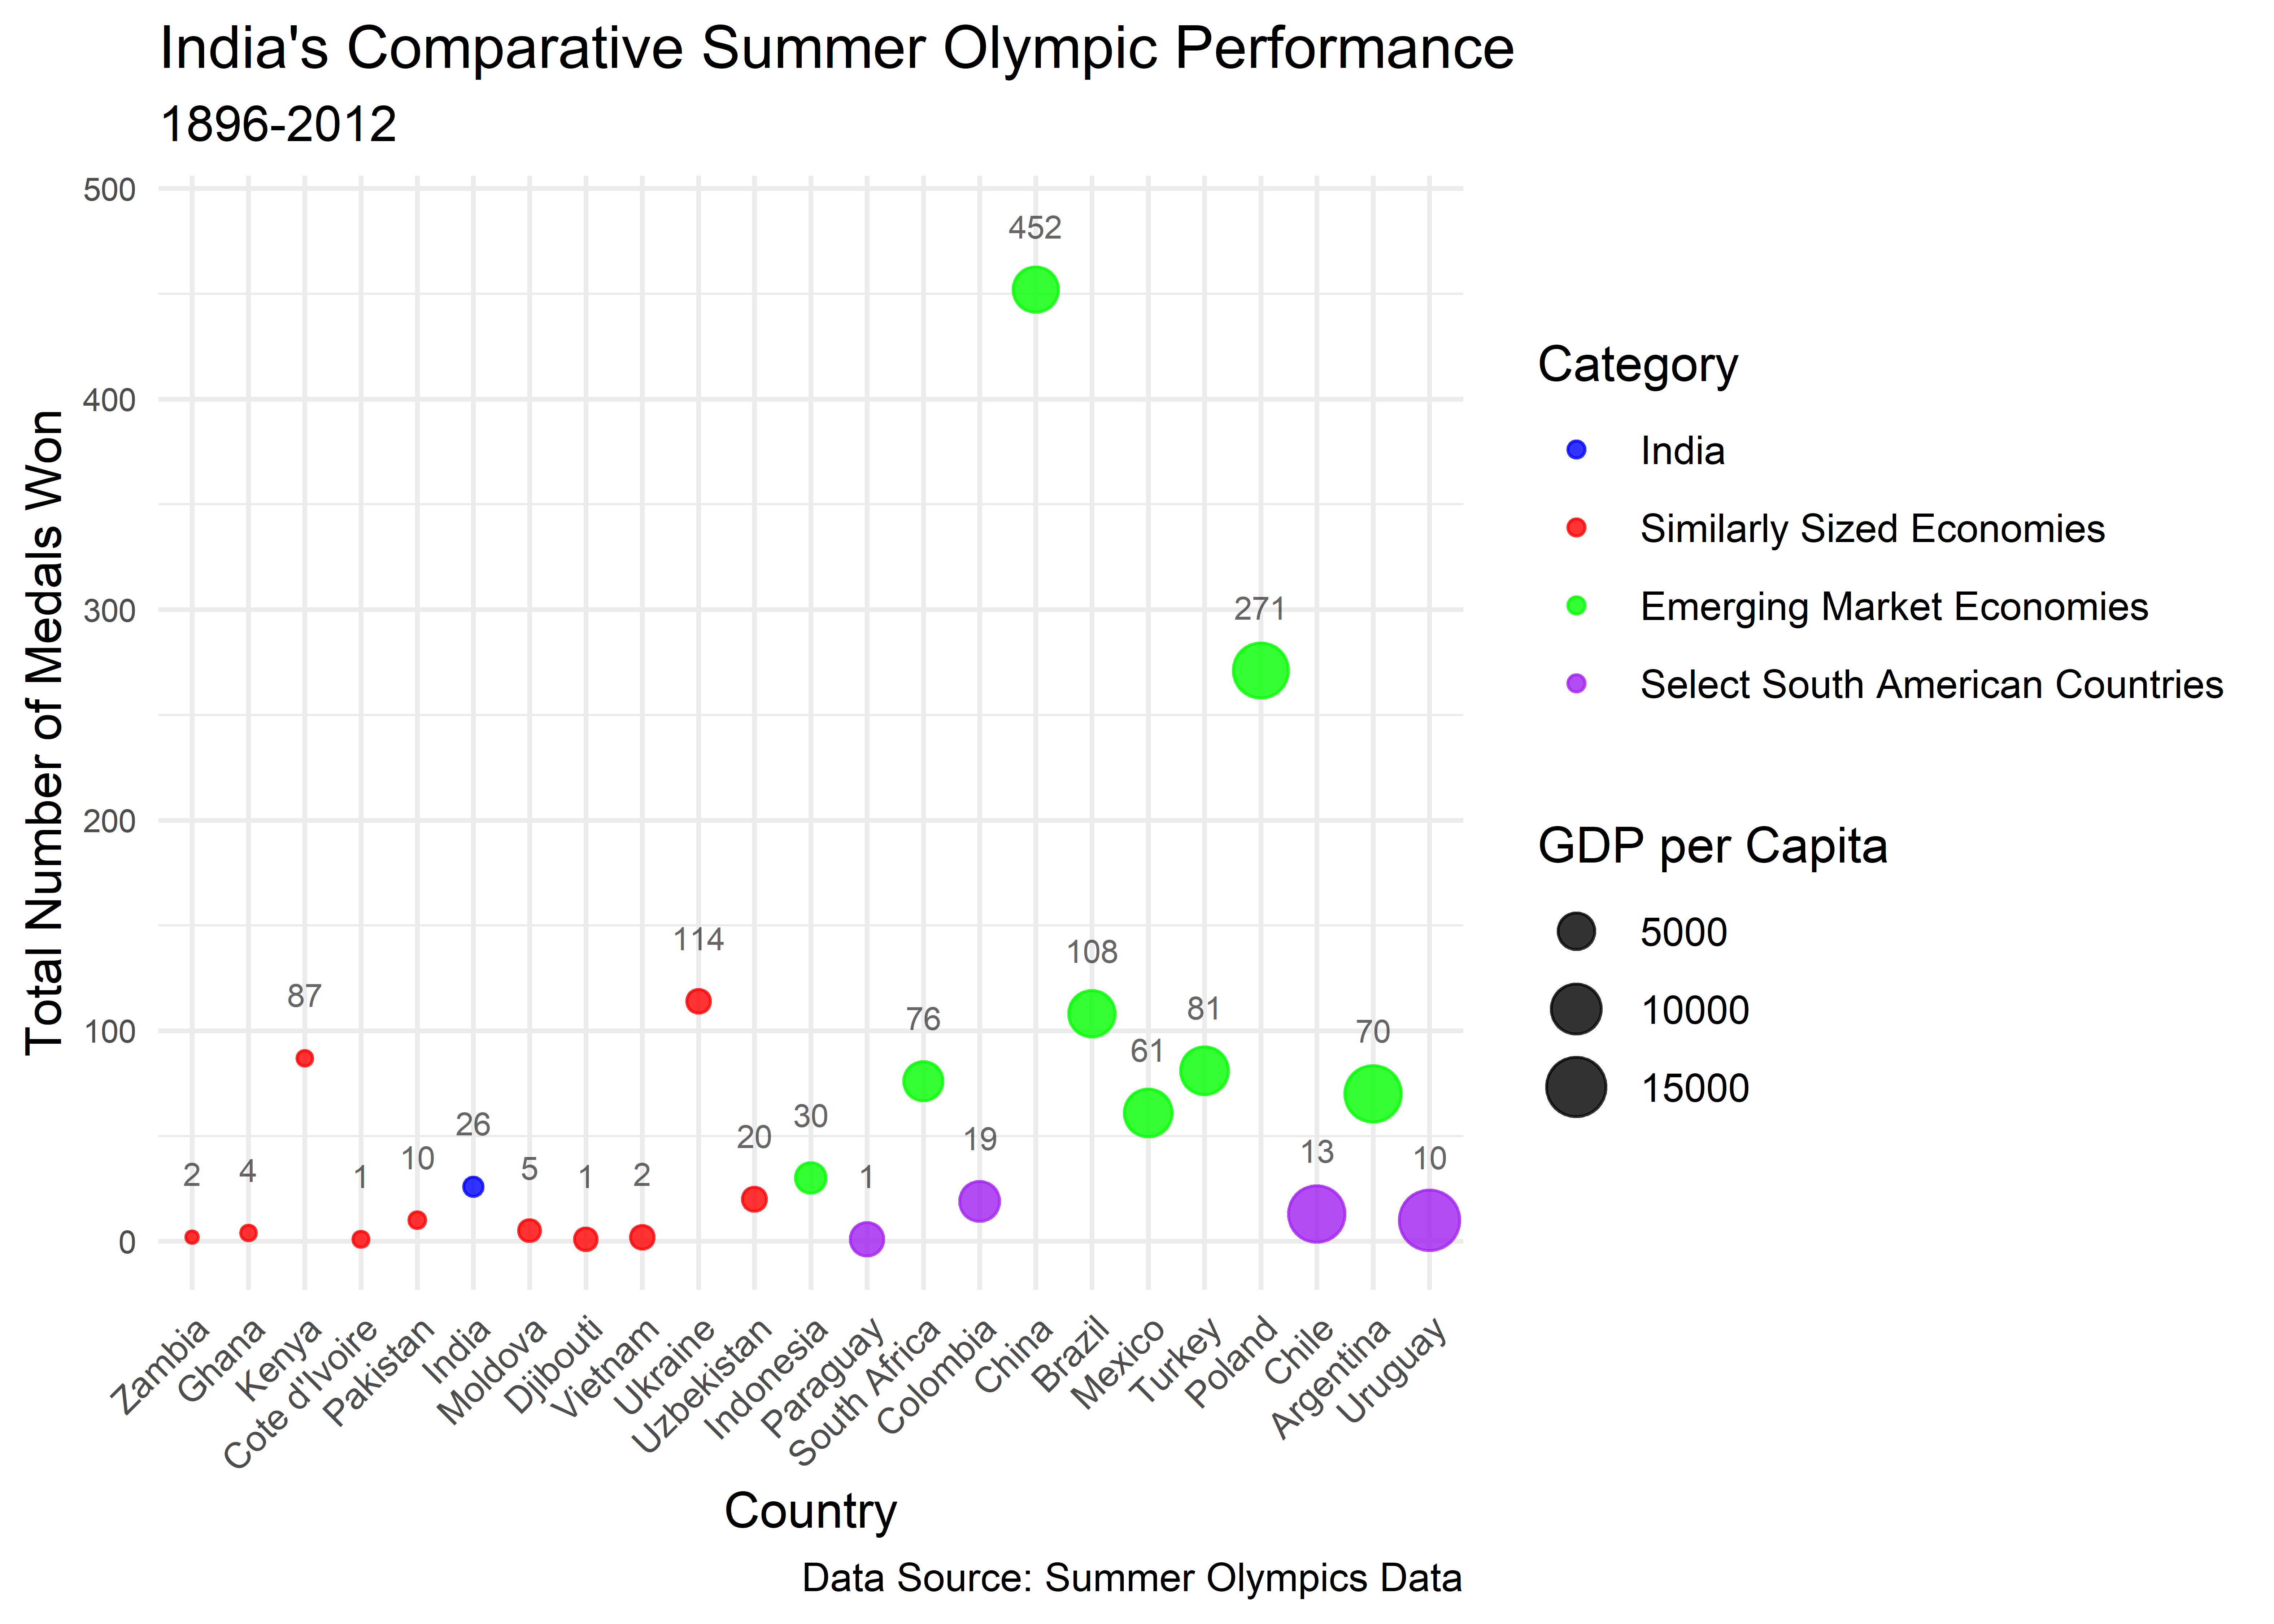
\includegraphics{Question_4_files/figure-latex/Figure1-1} 

}

\caption{India's Comparative Performance \label{Figure1}}\label{fig:Figure1}
\end{figure}

\newpage

\hypertarget{the-dominant-countries-over-time-in-both-summer-and-winter-olympics}{%
\section{\texorpdfstring{The Dominant Countries Over Time in Both Summer
and Winter Olympics
\label{dominate}}{The Dominant Countries Over Time in Both Summer and Winter Olympics }}\label{the-dominant-countries-over-time-in-both-summer-and-winter-olympics}}

This ssection aims to show which countries have been most dominant in
both the Winter and Summer Olympics over time. The plot shows the
cumulative total number of medals every year, amongst 8 countries who
have received more than 50 medals in any given year. The figure
highlights that:

\begin{itemize}
\item
  While China and Russia have shown exponentially growth in the number
  of medals won, this performance has only occurred post-1980,
  emphasising that it is really the other 6 countries, namely the US,
  UK, Germany, Sweden, France and Australia, that have dominated the
  olympics over time.
\item
  The US are by far the most dominant, with large numbers of medal
  winnings every Olympics.
\item
  China and Russia despite only starting to win since the 1980s, have
  virtually caught up to Australia and Sweden in terms of total medals
  won.
\end{itemize}

\begin{figure}[H]

{\centering 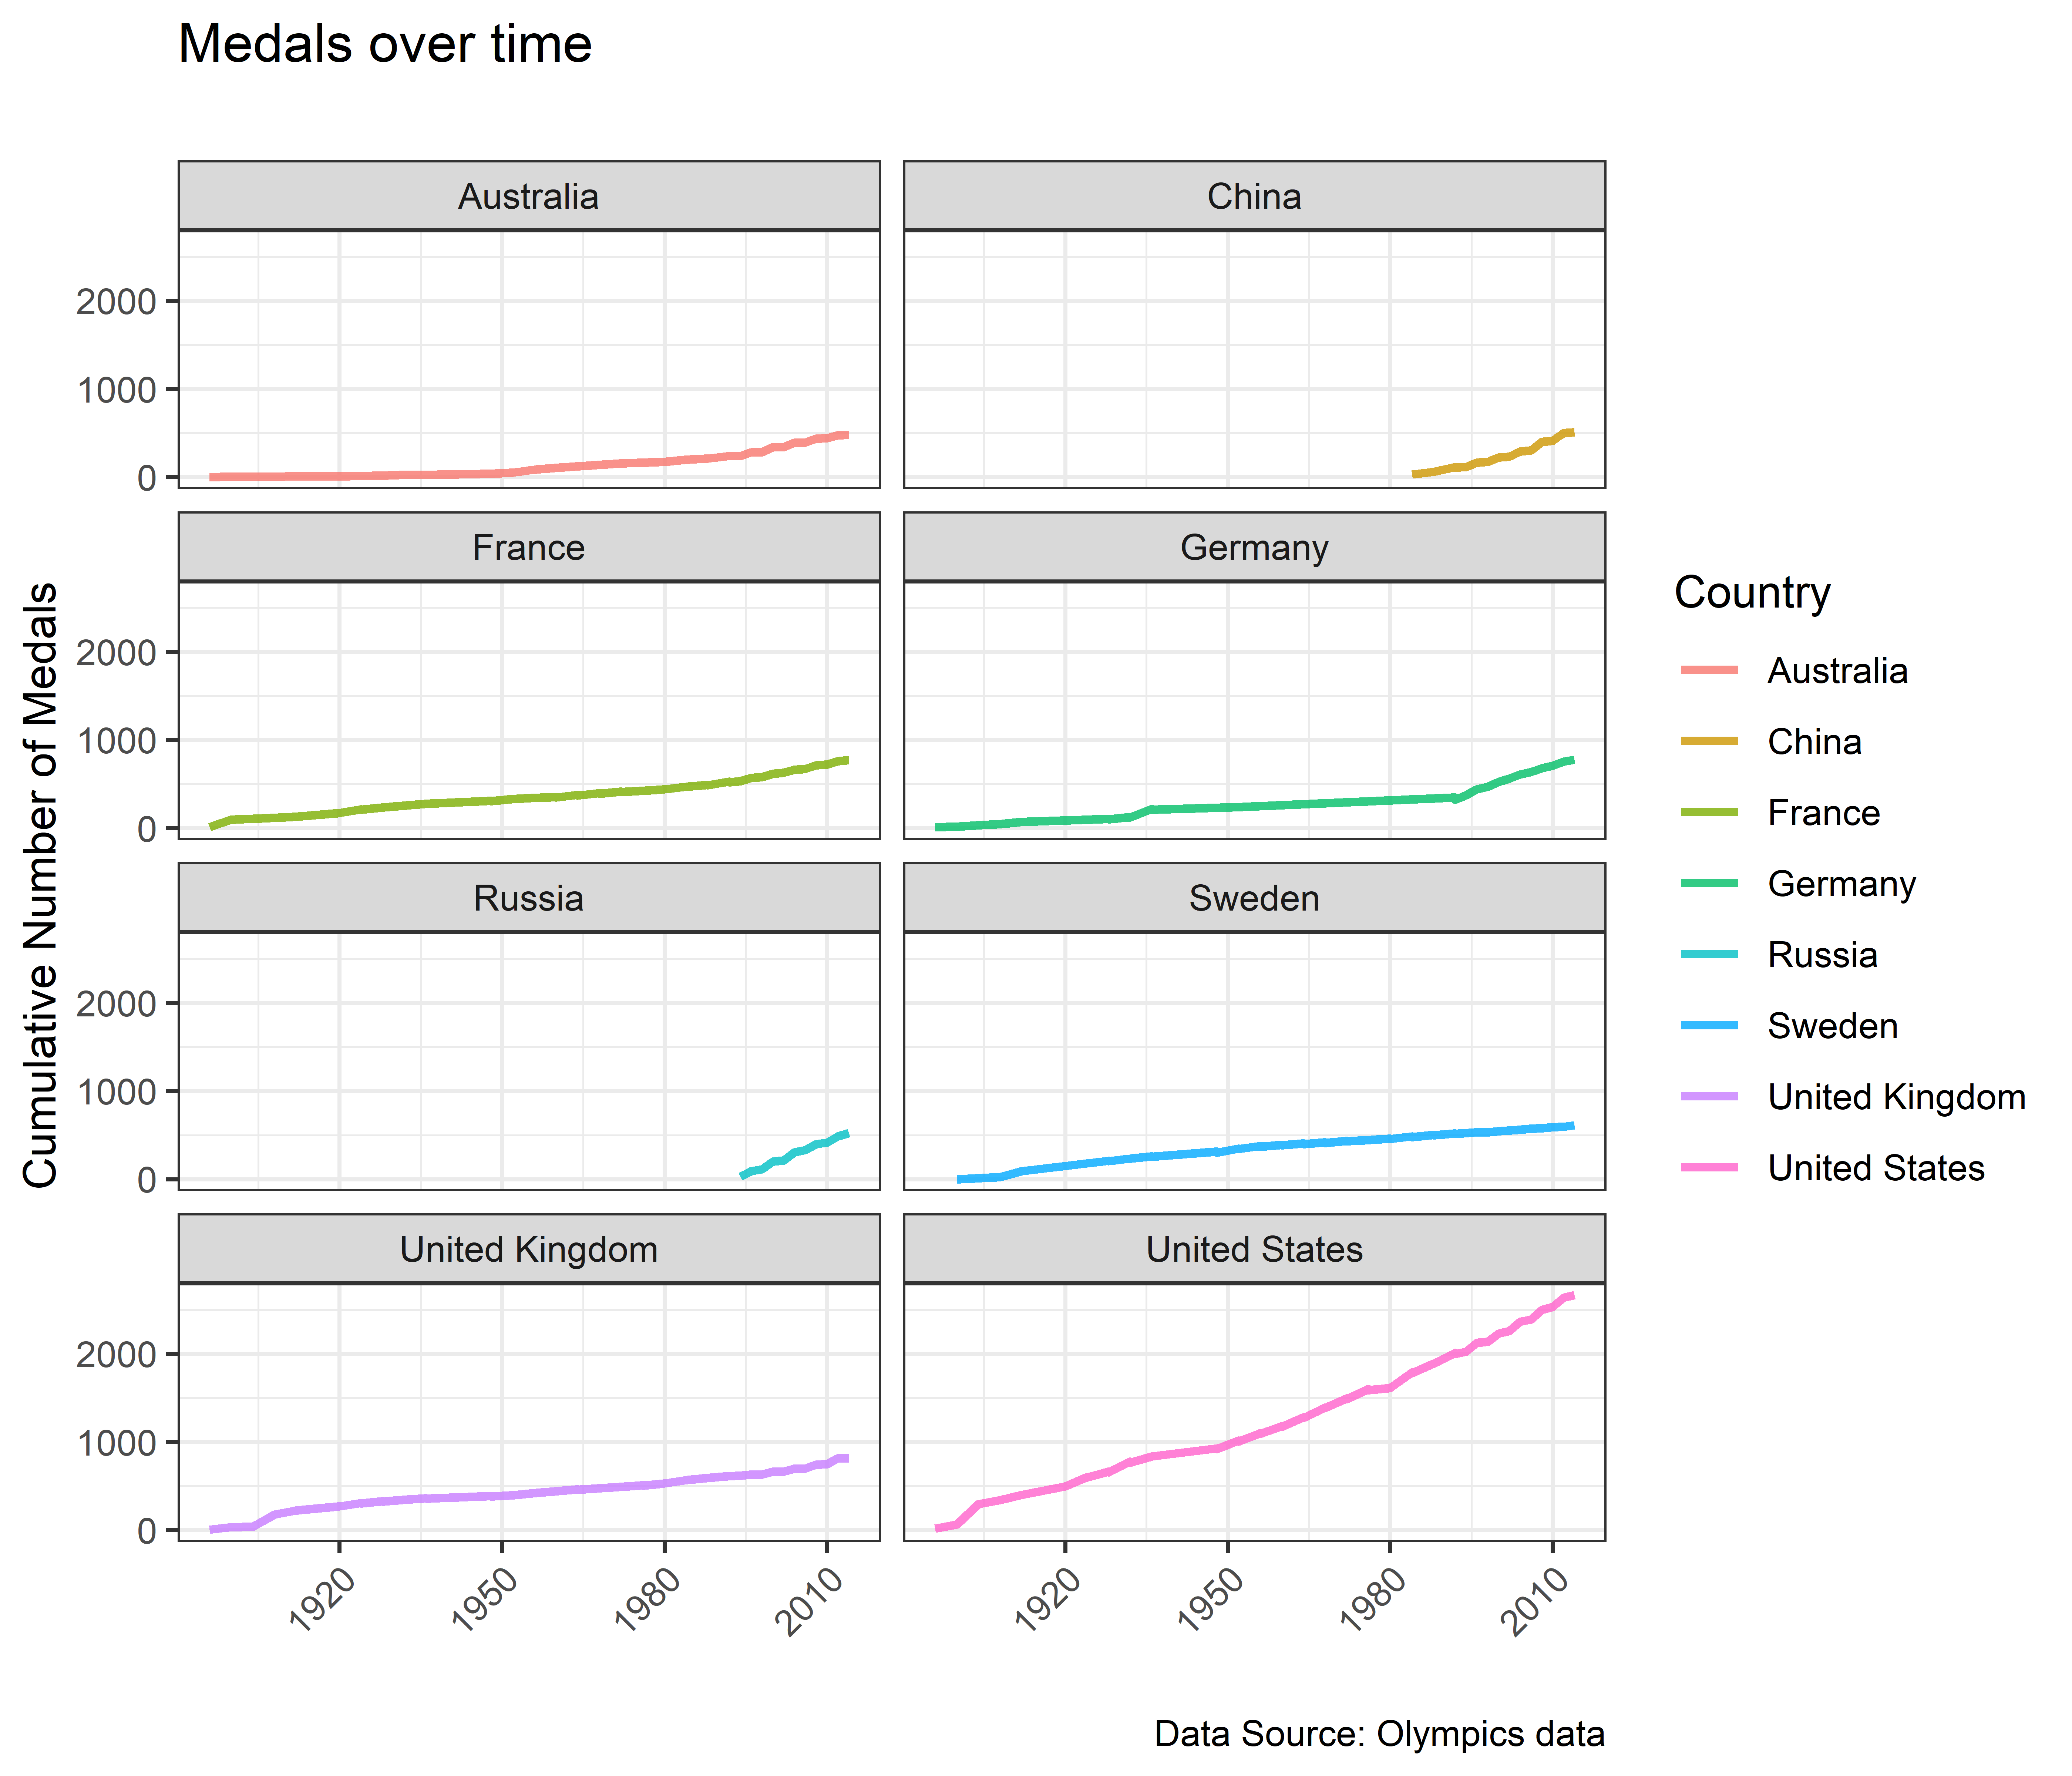
\includegraphics{Question_4_files/figure-latex/Figure2-1} 

}

\caption{Dominant Countries Cumulative Performance Over Time \label{Figure2}}\label{fig:Figure2}
\end{figure}

\newpage

\hypertarget{the-countries-punching-above-their-weight}{%
\section{\texorpdfstring{The Countries Punching Above Their Weight
\label{punching}}{The Countries Punching Above Their Weight }}\label{the-countries-punching-above-their-weight}}

In the figures below, the aim is to show which countries ``best punch
above their weight'' when it comes to winning medals. We focus on two
things: which countries have a small overall population, and which
countries have small overall GDP per Capita, but win many medals in the
Olympics.

\begin{itemize}
\item
  Figure \ref{Figure3} capturing Population vs Total Medals shows that
  Sweden is doing particularly well in the Olympics despite a small
  population, as are Canada, Australia, Hungary, Norway and Finland.
\item
  Figure \ref{Figure4}, which captures GDP per Capita vs Total Medals,
  shows that Hungary, Russia and China are doing well despite low GDP
  per Capita. Similarly, while Bulgaria and Poland have not amassed more
  than 400 medals, they have over 200 despite a GDP/capita less than
  \$20 000.
\item
  Thus, it appears that Hungary have done well historically despite a
  comparatively smaller population and lower GDP/capita.
\end{itemize}

\begin{figure}[H]

{\centering 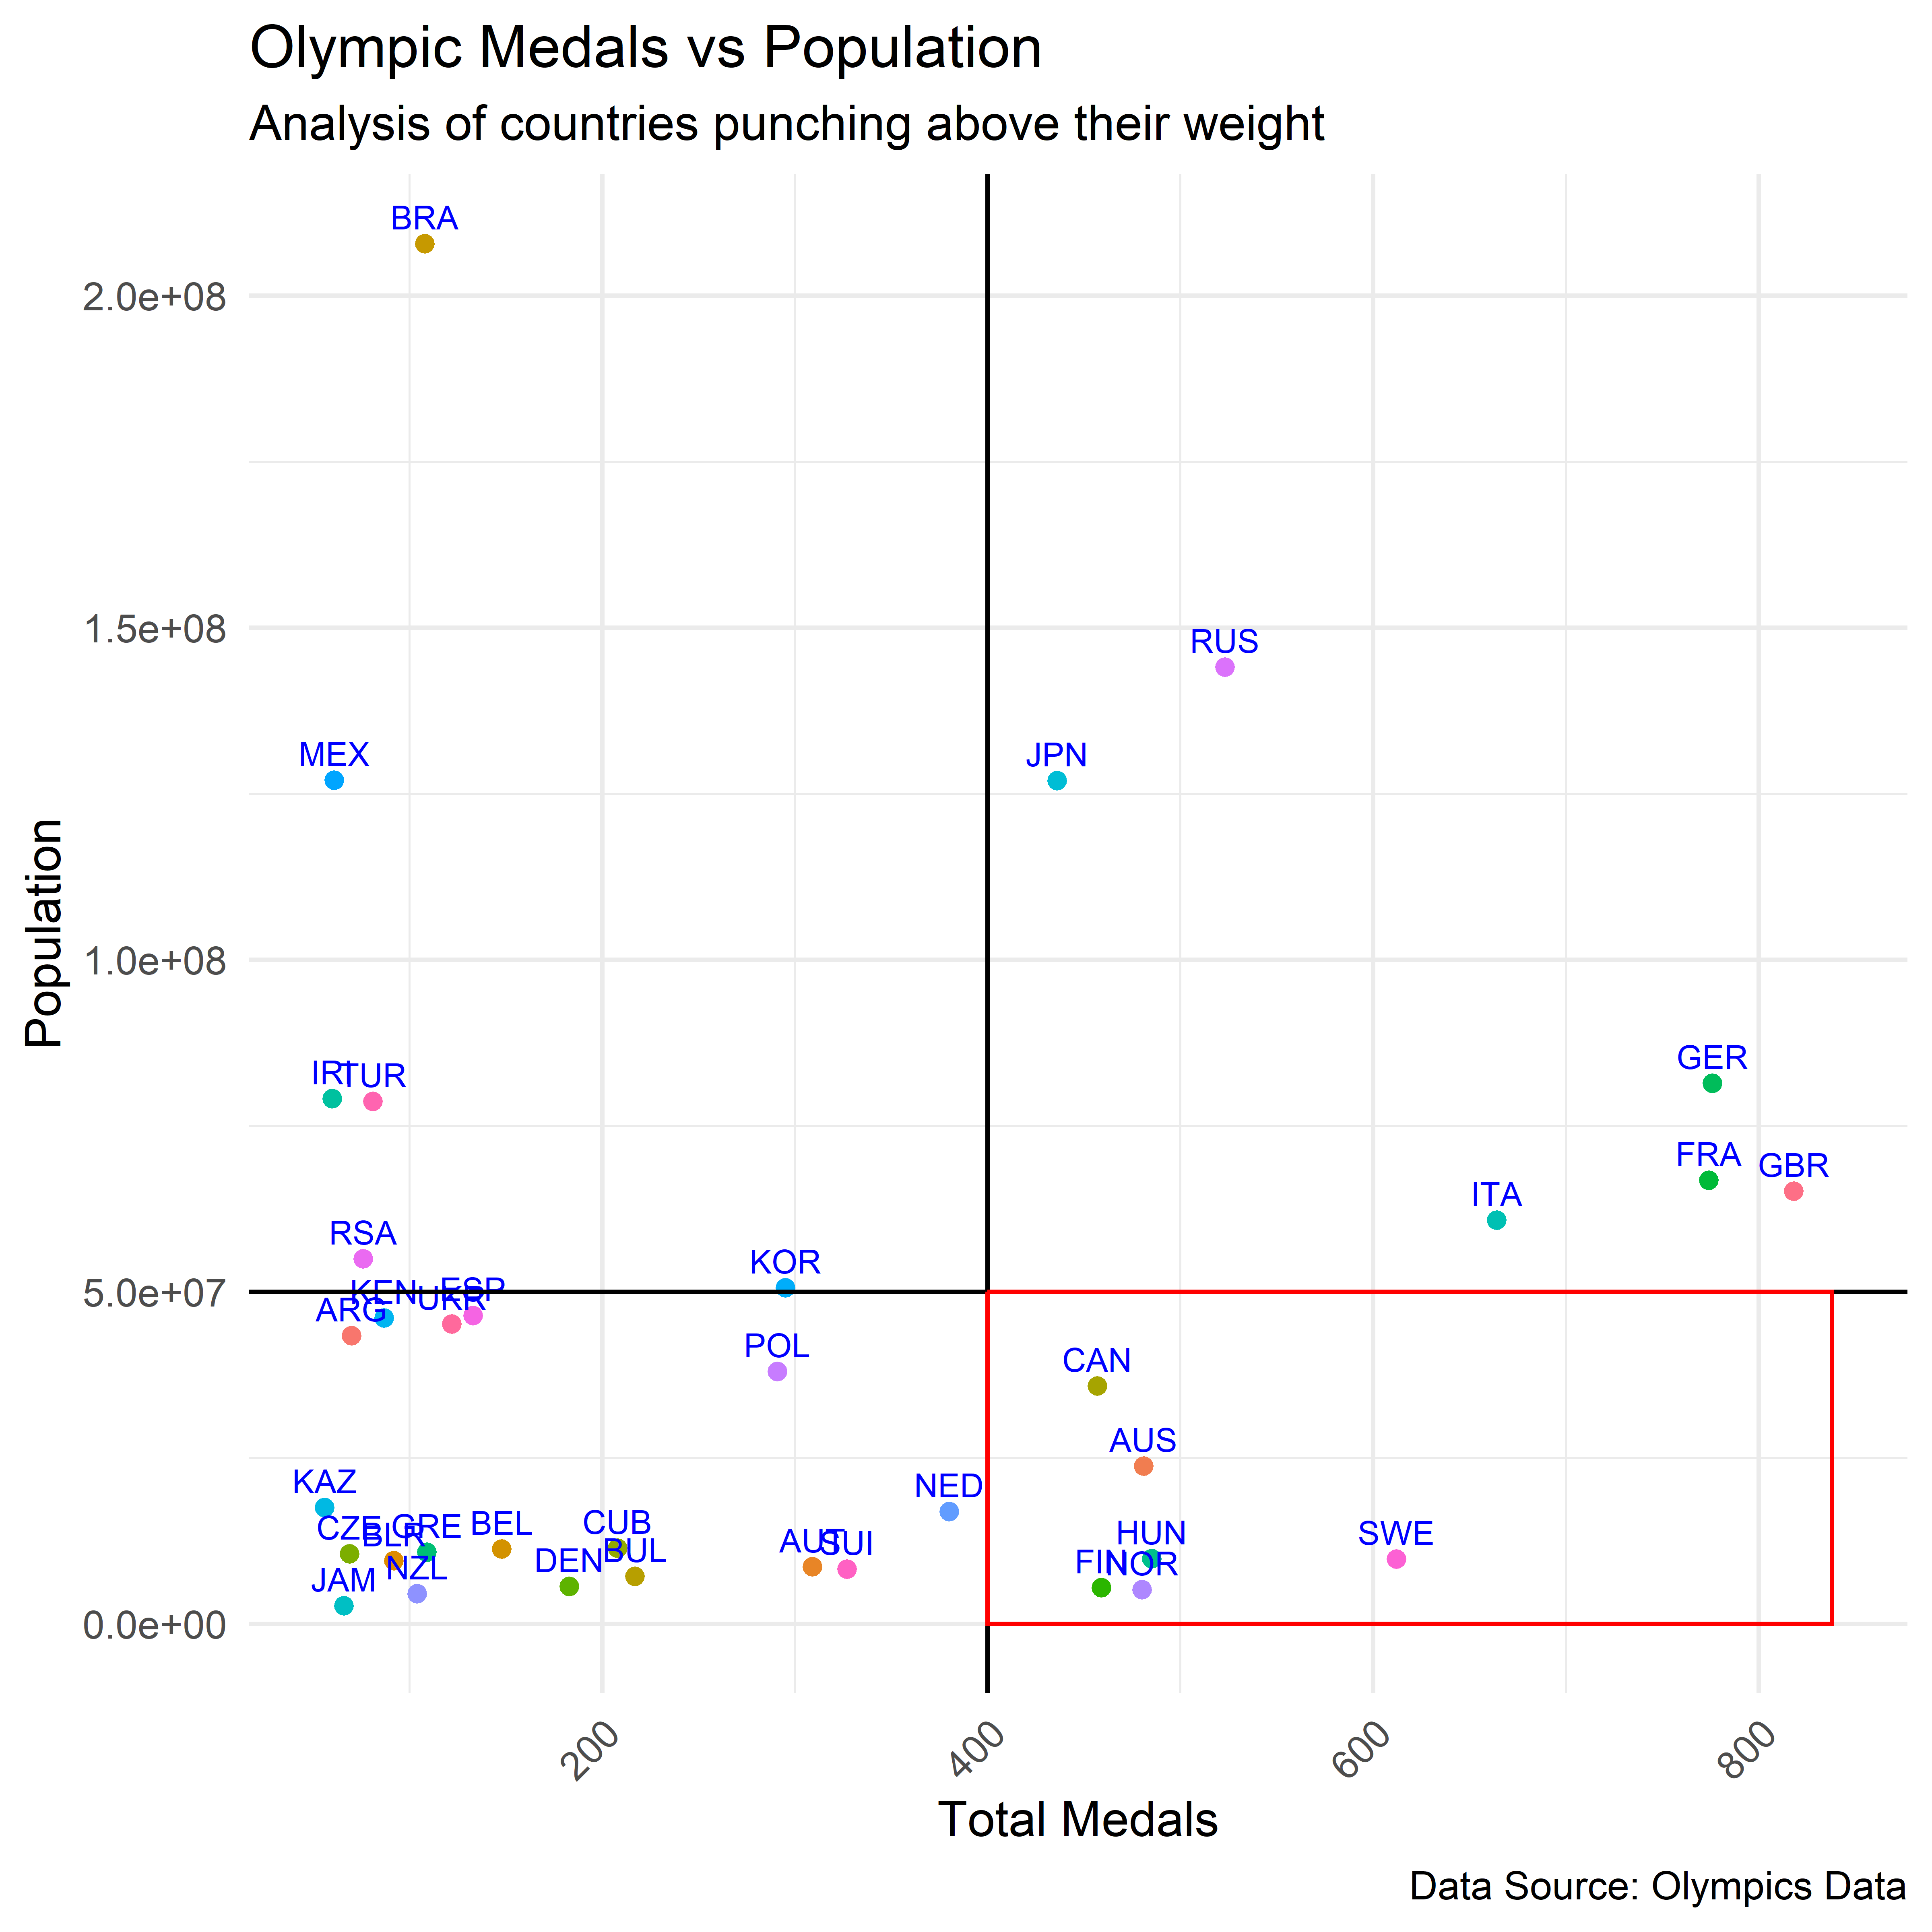
\includegraphics{Question_4_files/figure-latex/Figure3-1} 

}

\caption{Punching above Population Size \label{Figure3}}\label{fig:Figure3}
\end{figure}

\begin{figure}[H]

{\centering 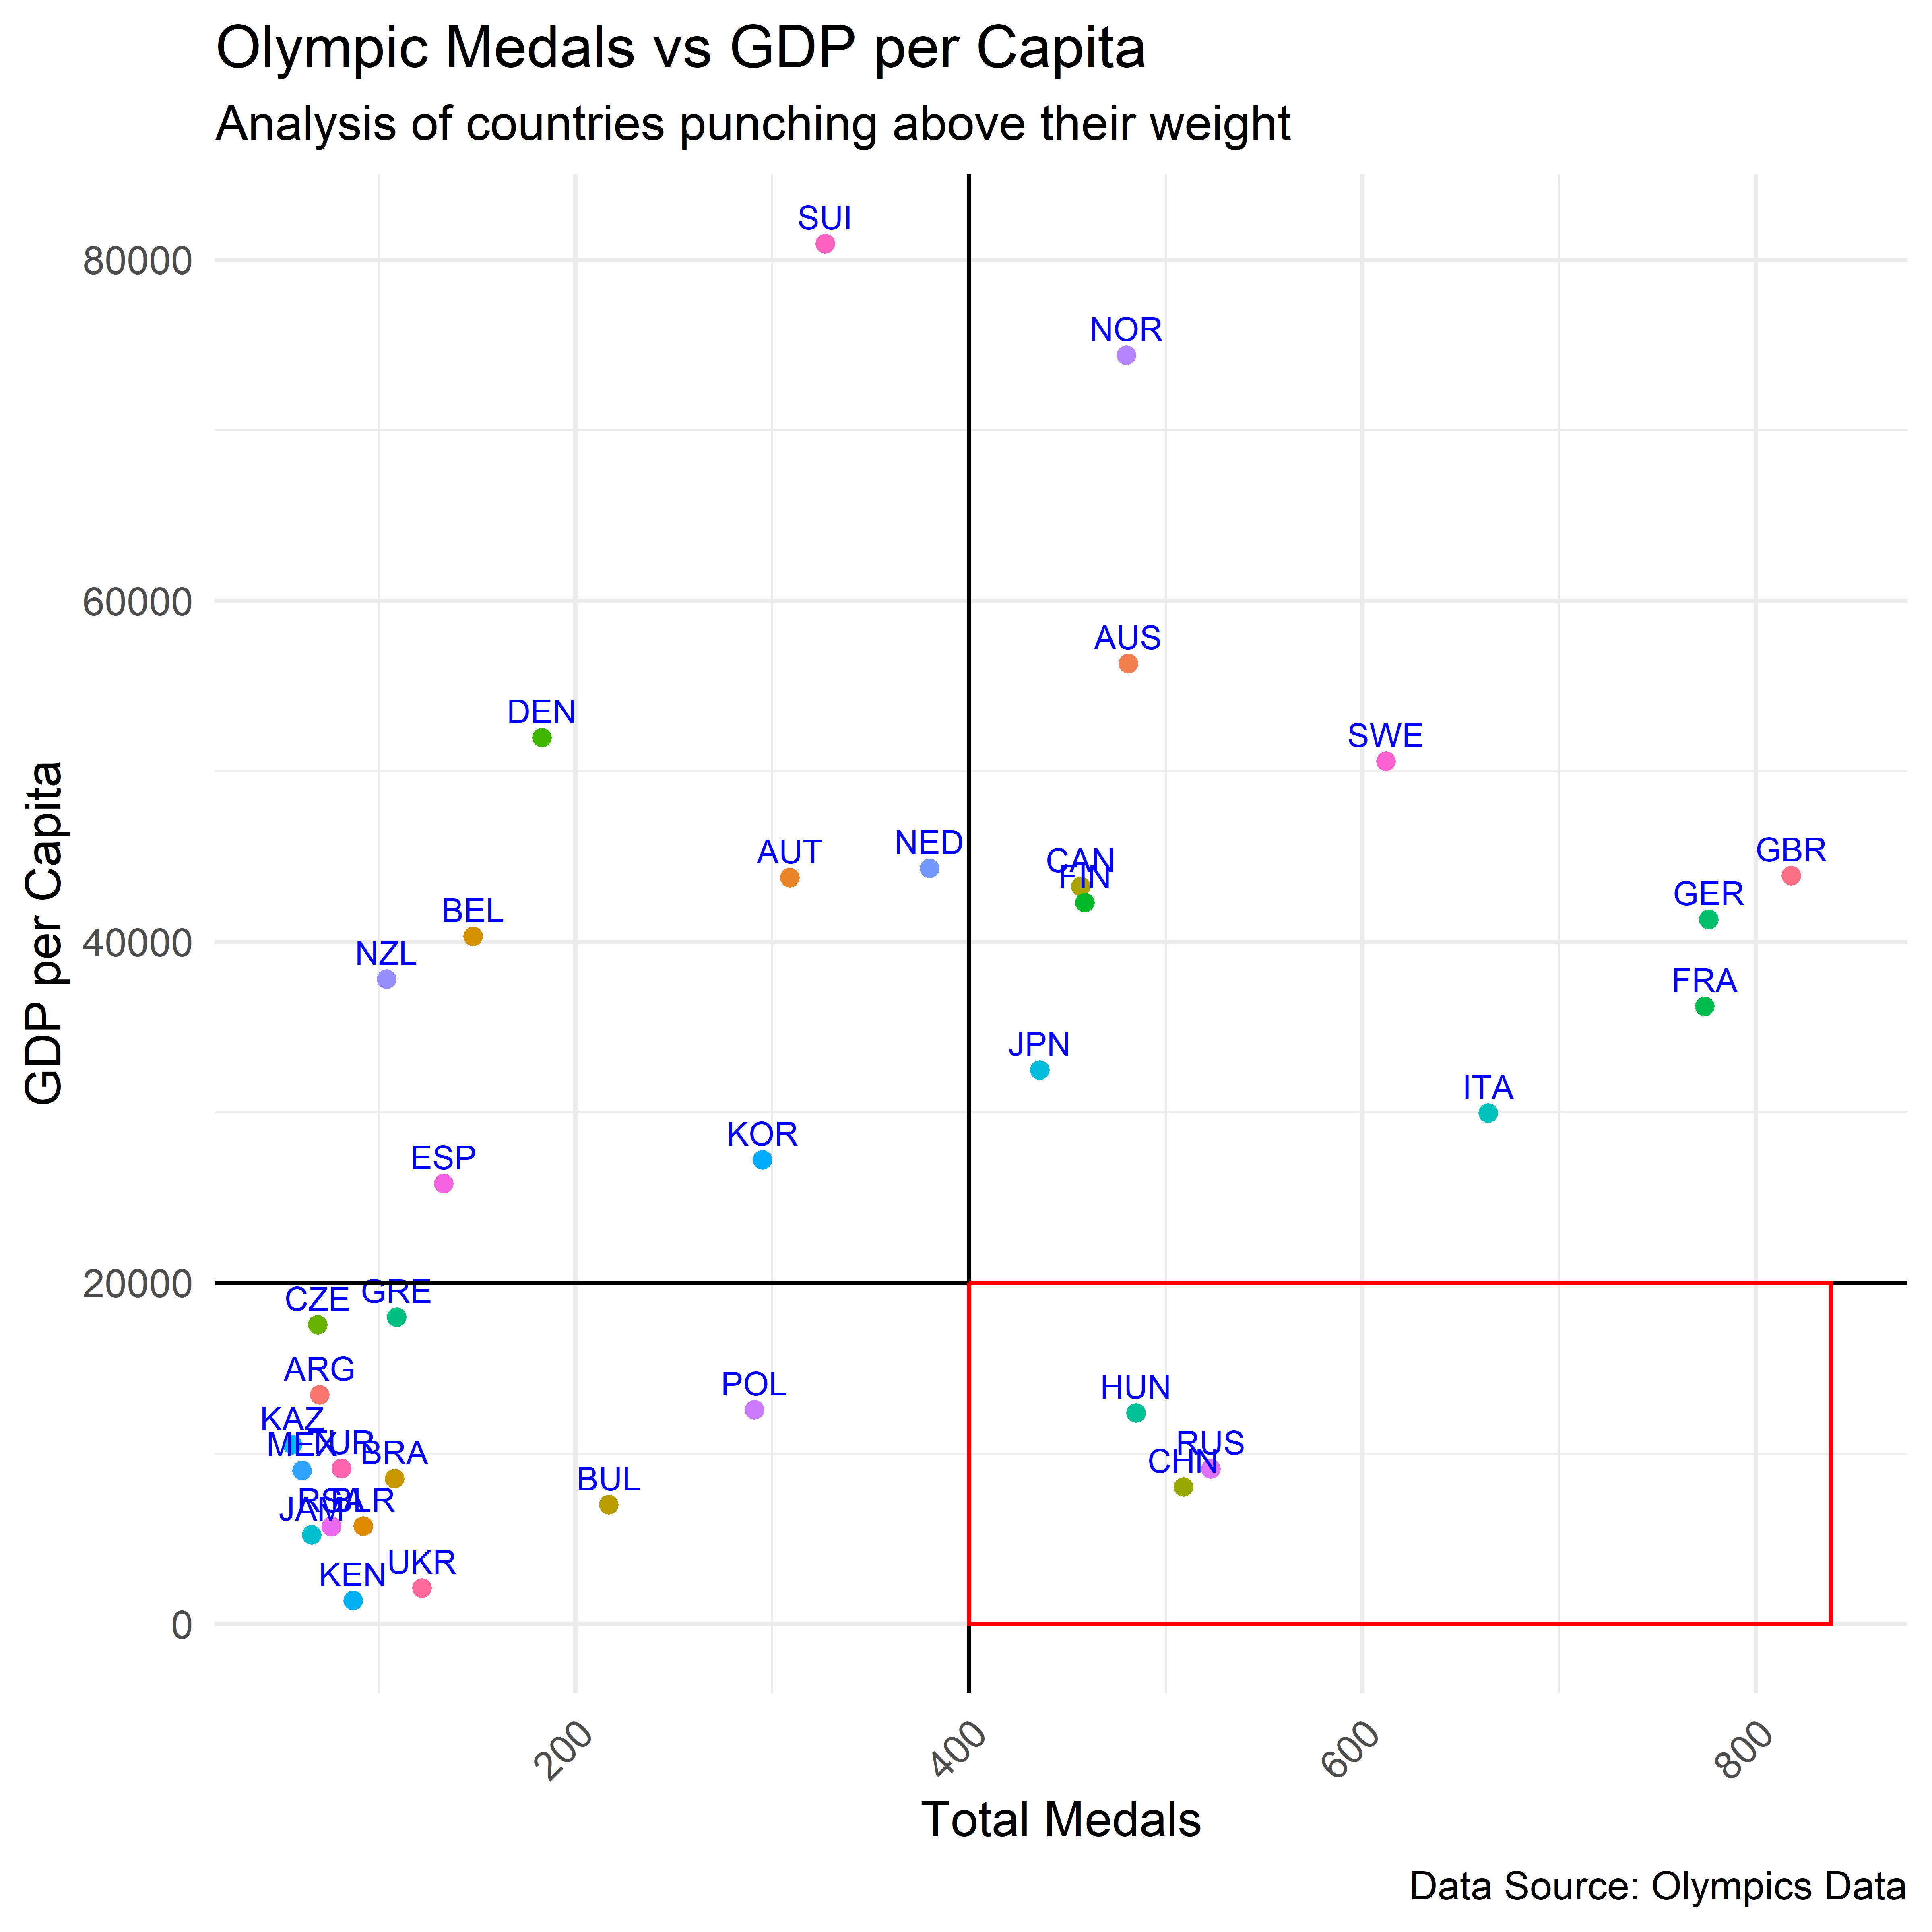
\includegraphics{Question_4_files/figure-latex/Figure4-1} 

}

\caption{Punching above Economy Size \label{Figure4}}\label{fig:Figure4}
\end{figure}

\hypertarget{my-favourite-events}{%
\section{\texorpdfstring{My Favourite Events
\label{my_events}}{My Favourite Events }}\label{my-favourite-events}}

My favourite event at the Olympics is the track events, particularly
middle and long distance, so the 800m and 1500m Track.

The plot below highlights how: * The US dominates the Gold Medal wins
for the 800m. * The UK take some of the gold medals from the US in the
800m. * The UK dominate the gold medal wins for the 1500m. * Kenya
enters as a strong contender in the 1500m. * New Zealand and Algeria
emerge as gold medal winners in the 1500m.

\begin{figure}[H]

{\centering 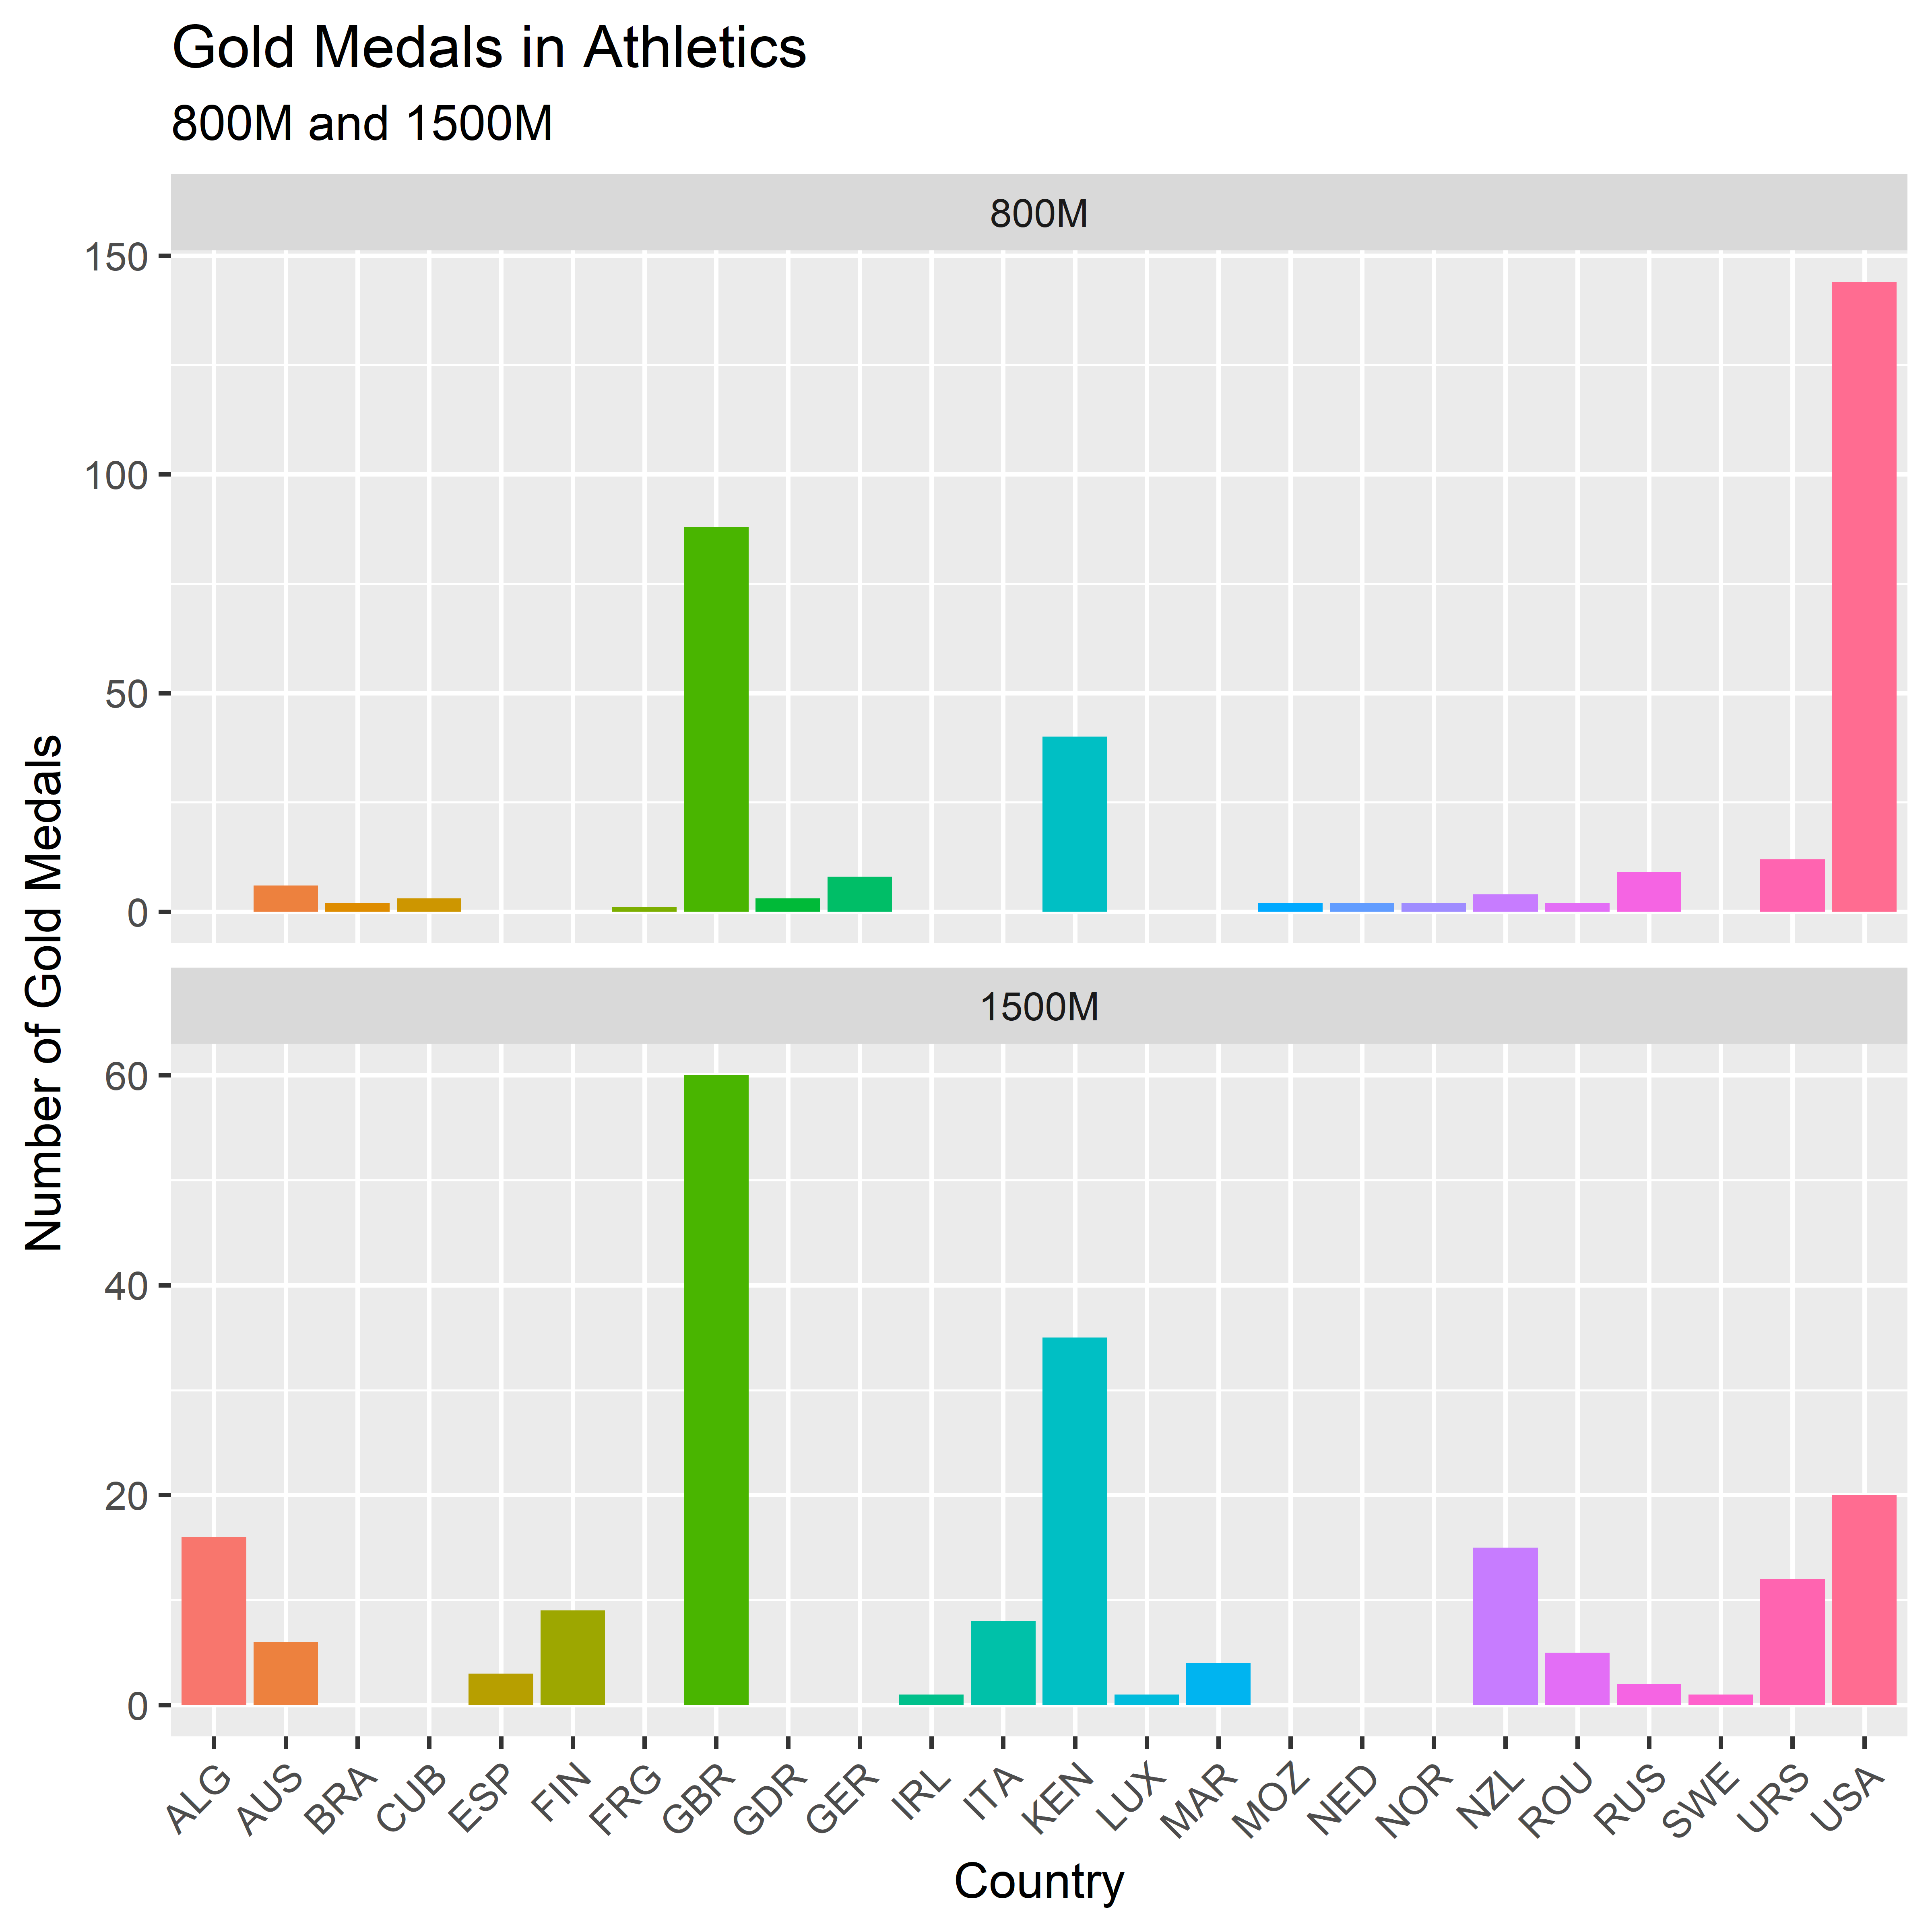
\includegraphics{Question_4_files/figure-latex/Figure5-1} 

}

\caption{800m and 1500m Gold Medalists \label{Figure5}}\label{fig:Figure5}
\end{figure}

\newpage

\hypertarget{references}{%
\section*{References}\label{references}}
\addcontentsline{toc}{section}{References}

\hypertarget{refs}{}
\begin{CSLReferences}{1}{0}
\leavevmode\vadjust pre{\hypertarget{ref-sankaran2021does}{}}%
Sankaran, A., Krishna, A. \& Vadivel, A. 2021. How does manufacturing
output affect export behaviors in emerging market economies? Evidence
from a dynamic panel ARDL for ten biggest emerging market economies.
\emph{Future Business Journal}. 7(1):26.

\end{CSLReferences}

\bibliography{Tex/ref}





\end{document}
